%
% normalnilp.tex
%
% (c) 2021 Prof Dr Andreas Müller, OST Ostschweizer Fachhochschule
%
\bgroup
\definecolor{darkgreen}{rgb}{0,0.6,0}
\def\sx{1.9}
\def\sy{0.6}
\def\punkt#1#2#3{
	\foreach \y in {0,...,#2}{
	}
}
\def\block#1#2{
	\fill[rounded corners=2pt,color=white]
		({-#1*\sx-0.4},-0.05) rectangle ({-#1*\sx+0.4},{#2*\sy+0.05});
	\draw[rounded corners=2pt]
		({-#1*\sx-0.4},-0.05) rectangle ({-#1*\sx+0.4},{#2*\sy+0.05});
}
\def\teilmenge#1#2#3{
	\fill[rounded corners=2pt,color=white]
		({-#1*\sx-0.35},{#2*\sy}) rectangle ({-#1*\sx+0.35},{#3*\sy+0.00});
	\draw[rounded corners=2pt,color=gray]
		({-#1*\sx-0.35},{#2*\sy}) rectangle ({-#1*\sx+0.35},{#3*\sy+0.00});
}
\def\rot#1#2#3{
	\fill[rounded corners=2pt,color=red!20]
		({-#1*\sx-0.35},{#2*\sy+0.00})
			rectangle ({-#1*\sx+0.35},{#3*\sy+0.00});
	\draw[rounded corners=2pt,color=red]
		({-#1*\sx-0.35},{#2*\sy+0.00})
			rectangle ({-#1*\sx+0.35},{#3*\sy+0.00});
}
\def\hellblau#1#2#3{
	\fill[rounded corners=2pt,color=blue!20]
		({-#1*\sx-0.35},{#2*\sy+0.00})
			rectangle ({-#1*\sx+0.35},{#3*\sy+0.00});
	\draw[rounded corners=2pt,color=blue!40]
		({-#1*\sx-0.35},{#2*\sy+0.00})
			rectangle ({-#1*\sx+0.35},{#3*\sy+0.00});
}
\def\punkt#1#2{
	\fill[color=blue] ({-#1*\sx},{(#2-0.5)*\sy}) circle[radius=0.08];
}
\def\bildpunkt#1#2{
	\fill[color=blue!40] ({-#1*\sx},{(#2-0.5)*\sy}) circle[radius=0.08];
}
\def\pfeil#1#2#3{
	\draw[->,color=blue,shorten >= 0.1cm,shorten <= 0.1cm] 
	({-#1*\sx},{(#2-0.5)*\sy}) 
	--
	({-(#1-1)*\sx},{(#3-0.5)*\sy}) ;
}
\begin{frame}[t]
\frametitle{Normalform einer nilpotenten Matrix}
{\usebeamercolor[fg]{title}$A^l=0$ $\Rightarrow$ finde eine ``gute'' Basis}
\begin{columns}[t,onlytextwidth]
\begin{column}{0.48\textwidth}
\vspace{-25pt}
\begin{center}
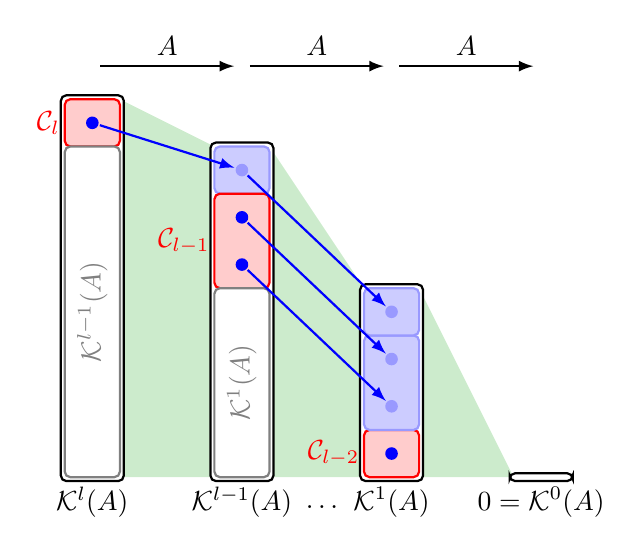
\begin{tikzpicture}[>=latex,thick]

\fill[color=darkgreen!20,rounded corners=2pt]
	({-3*\sx+0.35},0) -- (-0.35,0)
	--
	({-1*\sx+0.35},{4*\sy}) -- ({-1*\sx-0.35},{4*\sy})
	--
	({-2*\sx+0.35},{7*\sy}) -- ({-2*\sx-0.35},{7*\sy})
	--
	({-3*\sx+0.35},{8*\sy}) -- cycle;

\block{0}{0}

\block{1}{4}
\uncover<10->{
	\rot{1}{0}{1}
	\node[color=red] at ({-1*\sx-0.28},{0.5*\sy}) [left] {$\mathcal{C}_{l-2}$};
}
\uncover<8->{
	\hellblau{1}{1}{3}
}
\uncover<4->{
	\hellblau{1}{3}{4}
}

\block{2}{7}
\uncover<4->{
	\hellblau{2}{6}{7}
}
\uncover<6->{
	\rot{2}{4}{6}
	\node[color=red] at ({-2*\sx-0.28},{5*\sy}) [left] {$\mathcal{C}_{l-1}$};
}
\teilmenge{2}{0}{4}

\block{3}{8}
\uncover<2->{
	\rot{3}{7}{8}
	\node[color=red] at ({-3*\sx-0.28},{7.5*\sy}) [left] {$\mathcal{C}_l$};
}
\teilmenge{3}{0}{7}

\uncover<3->{
	\punkt{3}{8}
}
\uncover<4->{
	\pfeil{3}{8}{7}
	\bildpunkt{2}{7}
	\pfeil{2}{7}{4}
	\bildpunkt{1}{4}
}

\uncover<7->{
	\punkt{2}{5}
	\punkt{2}{6}
}
\uncover<8->{
	\pfeil{2}{5}{2}
	\bildpunkt{1}{3}
	\pfeil{2}{6}{3}
	\bildpunkt{1}{2}
}

\uncover<11->{
\punkt{1}{1}
}

\node at ({-3*\sx},0) [below] {$\mathcal{K}^l(A)\mathstrut$};
\node at ({-2*\sx},0) [below] {$\mathcal{K}^{l-1}(A)\mathstrut$};
\node at ({-1.45*\sx},0) [below] {$\dots\mathstrut$};
\node at ({-1*\sx},0) [below] {$\mathcal{K}^1(A)\mathstrut$};
\node at ({-0*\sx},0) [below] {$0=\mathcal{K}^0(A)\mathstrut$};
\node[color=gray] at ({-2*\sx},{2*\sy}) [rotate=90] {$\mathcal{K}^1(A)$};
\node[color=gray] at ({-3*\sx},{3.5*\sy}) [rotate=90] {$\mathcal{K}^{l-1}(A)$};
\foreach \x in {0,1,2}{
	\draw[->,shorten >= 0.1cm, shorten <= 0.1cm]
		({-(\x+1)*\sx},{8.7*\sy}) -- ({-(\x)*\sx},{8.7*\sy});
	\node at ({-(\x+0.5)*\sx},{8.7*\sy}) [above] {$A$};
}
\end{tikzpicture}
\end{center}
\end{column}
\begin{column}{0.48\textwidth}
\vspace{-30pt}
\begin{enumerate}
\item<2->	\(
	\mathcal{K}^l(A)=\mathcal{K}^{l-1}\oplus {\color{red}\mathcal{C}_l}
	\)
\item<3->	\(
	{\color{blue}b_1}\in{\color{red}\mathcal{C}_l}
	\)
\item<4->	\(
	\mathcal{B}_l
	=
	\{{\color{blue}b_1},{\color{blue!40}Ab_1},{\color{blue!40}A^2b_1},\dots,
	{\color{blue!40}A^{l-1}b_1}\}
	\)
\item<5->	\(
	\mathcal{K}^{l-1}(A)
	=
	\mathcal{K}^{l-2}(A)
	\oplus
	{\color{red}\mathcal{C}_{l-1}}
	\oplus
	{\color{blue}A\mathcal{C}_l}
	\)
\item<6->	\(
	{\color{blue}b_2},{\color{blue}b_3}\in{\color{red}\mathcal{C}_{l-1}}
	\)
\item<7->	\(
	\mathcal{B}_{l-1}
	=
	\{
	{\color{blue}b_2},{\color{blue}b_3},
	{\color{blue!40}Ab_2}, {\color{blue!40}Ab_3},\dots
	\}
	\)
\item<8-> \dots
\end{enumerate}
\begin{center}
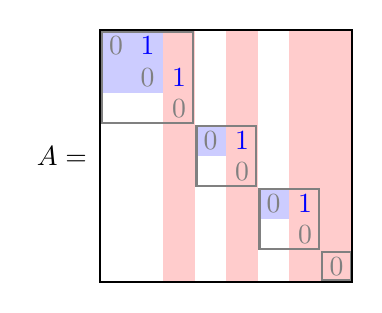
\begin{tikzpicture}[>=latex,thick,scale=0.4]

\uncover<2-4>{
	\fill[color=red!20] (2,0) rectangle (3,8);
}
\uncover<4->{
	\fill[color=blue!20] (0,6) rectangle (2,8);
}
\uncover<5->{
	\fill[color=red!20] (2,5) rectangle (3,8);
	\node[color=blue] at (2.5,6.5) {$1$};
	\node[color=blue] at (1.5,7.5) {$1$};
	\node[color=gray] at (0.5,7.5) {$0$};
	\node[color=gray] at (1.5,6.5) {$0$};
	\node[color=gray] at (2.5,5.5) {$0$};
	\draw[color=gray] (0.05,5.05) rectangle (2.95,7.95);
}

\uncover<6-8>{
	\fill[color=red!20] (4,0) rectangle (5,8);
	\fill[color=red!20] (6,0) rectangle (7,8);
}
\uncover<8->{
	\fill[color=blue!20] (3,4) rectangle (4,5);
	\fill[color=blue!20] (5,2) rectangle (6,3);
}
\uncover<9->{
	\fill[color=red!20] (4,3) rectangle (5,5);
	\node[color=blue] at (4.5,4.5) {$1$};
	\node[color=gray] at (3.5,4.5) {$0$};
	\node[color=gray] at (4.5,3.5) {$0$};
	\draw[color=gray] (3.05,3.05) rectangle (4.95,4.95);
	\fill[color=red!20] (6,1) rectangle (7,3);
	\node[color=blue] at (6.5,2.5) {$1$};
	\node[color=gray] at (5.5,2.5) {$0$};
	\node[color=gray] at (6.5,1.5) {$0$};
	\draw[color=gray] (5.05,1.05) rectangle (6.95,2.95);
}

\uncover<10>{
	\fill[color=red!20] (7,0) rectangle (8,8);
}
\uncover<11->{
	\fill[color=red!20] (7,0) rectangle (8,1);
	\node[color=gray] at (7.5,0.5) {$0$};
	\draw[color=gray] (7.05,0.05) rectangle (7.95,0.95);
}

\draw (0,0) rectangle (8,8);
\node at (-0.1,4) [left] {$A=$};

\end{tikzpicture}
\end{center}
\end{column}
\end{columns}
\end{frame}
\egroup
